%
% File acl2018.tex
%
%% Based on the style files for ACL-2017, with some changes, which were, in turn,
%% Based on the style files for ACL-2015, with some improvements
%%  taken from the NAACL-2016 style
%% Based on the style files for ACL-2014, which were, in turn,
%% based on ACL-2013, ACL-2012, ACL-2011, ACL-2010, ACL-IJCNLP-2009,
%% EACL-2009, IJCNLP-2008...
%% Based on the style files for EACL 2006 by 
%%e.agirre@ehu.es or Sergi.Balari@uab.es
%% and that of ACL 08 by Joakim Nivre and Noah Smith

\documentclass[11pt,a4paper]{article}
\usepackage[hyperref]{acl2018}
\usepackage{times}
\usepackage{latexsym}
\usepackage{graphicx}
\usepackage{url}

\aclfinalcopy % Uncomment this line for the final submission
%\def\aclpaperid{***} %  Enter the acl Paper ID here

%\setlength\titlebox{5cm}
% You can expand the titlebox if you need extra space
% to show all the authors. Please do not make the titlebox
% smaller than 5cm (the original size); we will check this
% in the camera-ready version and ask you to change it back.

\newcommand\BibTeX{B{\sc ib}\TeX}

\title{Detecting Sarcasm Using NLP Techniques}

\author{Saul Grimaldo \\
  DATASCI W266\\
  UC Berkeley \\
  School of Information \\
  {\tt saul\char`_grimaldo@berkeley.edu} \\\And
  Ramsey Maga{\~n}a \\
  DATASCI W266\\
  UC Berkeley \\
  School of Information \\
  {\tt ramagana@berkeley.edu} \\}

\date{}

\begin{document}
\maketitle
\begin{abstract}
Due to the increasing importance of NLP, it's important now more than ever to detect linguistic phenomena that can often be subtle but which ignoring may result in costly mistakes in critical business usages. This paper attempts to provide a practical way of detecting sarcasm, a subtle linguistic phenomenon that often completely changes the meaning of the language used. 

We provide some background on models that are typically used for sarcasm detection which heavily rely on information that may be difficult to obtain for the typical business. We then provide a methodology using only the tweet to which a message is responding to to build context.

A Naive Bayes model that does not use context is used to set a performance benchmark for the main model we will focus on: the Bi CNN model. Both models performed well, but the Bi-CNN did not beat our baseline model, suggesting that the limitations in our sample size may be contributing to our model's performance. Additional caveats, which we describe later in this paper apply.

\end{abstract}

\section{Introduction}
Sarcasm is challenging to detect. Even the typical person may have difficulties distinguishing a non-sarcastic comment from a sarcastic one. Often times, a person requires context on the conversation to be able to confidently determine whether a statement is sarcastic. This makes sarcasm even more difficult for a machine learning algorithm to detect. However, sarcasm detection is critical in some applications. 

The field of sentiment analysis can often be critical for business attempting to grow using customer testimony to present prospective customers with happy users experience with their products. A sarcastic message may, however, slip through the cracks, providing a scathing review hidden by heavy sarcasm that uses highly positive language. Sarcasm is also important in detecting toxic messages. Often times toxic messages are delivered using sarcastic comments. In both cases, it's possible to use the immediate context without having to rely on user-level data.

Current techniques rely heavily on user history. That is, we must understand the user who's posting a message to understand if they are
being sarcastic. Some algorithms even require knowledge of the target audience as well. Properly capturing this information however, may be unwieldy and perhaps even unethical. 

We present a methodology that uses convolutional neural networks that rely only on the context in which the message was posted. We define context in two ways. First is what, if anything, a given tweet is responding to. To do this, we collected the immediately prior tweet to which the twitter message of interest is responding to if they were responding to anything. The second definition of context is the given topic that the tweet is covering. In twitter, we can gather this sort of contextual information through the use of hashtags.

We rely on data scraped through Twitter to build our models, using the \#sarcasm and \#sarcastic hashtags to label our training examples. We sample a set of popular hashtags as well to gather negative examples. This provides a fundamental issue. It's common for people to be sarcastic without using a hashtag announcing the fact. It's also possible that someone uses the sarcasm or sarcastic hashtags even when they are not being sarcastic. As such, our algorithm will  be built on an imperfect foundation. To more properly build this model out would require a team of annotators to determine whether a given tweet is sarcastic. However, even this method proved to be challenging for Davidov et al as their team of expert annotators were not completely certain whether a message should be labeled as sarcastic [1].

\section{Background}

Historical experiments in this space have sourced data from social media channels like twitter, utilizing hashtags for labeling sarcasm (e.g. \#sarcasm, \#sarcastic, \#not) as seen in the paper by Bamman and Smith. In the Bamman paper, logistic regression is used for classification by training the model with a combination of tweet, author and environmental features[2].  In a paper by Amir et al[3] they use user embeddings to help provide contextual features for their model.  Moreover, there have been more advanced approaches to detecting sarcasm by way of using CNNs + LSTM + DNN as seen in Ghosh and Veale[4].  Additionally some semi-supervised approaches are also used as done by Davidov et al[1]. We compare the performances of these models against ours in the results section.

\section{Methods}
Our objective is to predict whether a message is sarcastic or not. To measure the effectiveness of our methodology, we will be using the  F1-score , in a similar way as the authors discussed in the background section. 

Two key techniques are used to detect whether a given tweet is sarcastic or not: the baseline model, which is a Naive Bayes model using a bag of words, and the Bi Convolutional Neural Network model,  which uses the message of interest, and the message which is being responded to as the main set of features.

For the purpose of these experiments, a 70-20-10 training-validation-test split is performed on our data. 

\subsection{Data}
Similar to both the Ghosh \& Veale and the Bannam \& Smith papers, we utilize functionality provided by twitter to access twitter streams. Using the twitter streaming api for python, tweepy, we collect our positive and negative class examples, sarcastic and non-sarcastic respectively.  

To collect positive examples of sarcasm we used self-declared labels of sarcasm with the following the \#sarcasm and \#sarcastic hashtags.  An initial attempt also used the hashtag \#not, however the vast majority of tweets in this hashtag were not sarcastic, so they were removed from our analysis to get a cleaner look at the data. To collect negative examples of sarcasm we aimed to create sample that is representative of the Twitterspere population. Our negative hashtags were chosen by identifying the most active hashtags for the following categories:  gaming, sports, fun, science, non-profit, news, technology, music, politics, and lifestyle.  Across the 10 categories, we have included 194 unique hashtags in the filter the stream to collect the negative class.  

The tweet objects are received in JSON-like objects.  Features of the tweets that were of interest include user identification information, full text of the tweet including the hashtag labels, information connecting the tweet to any tweet (or status) and user that it is in reply to.  Lastly, additional attribute information to filter data set, such as language and geographical information. 

Because of the context we'll be working on in this problem involves people sending out the same message through various accounts through retweets, we chose to not remove a retweeted message as we will have access to the history of retweets in the context in which we envision this algorithm to de deployed in.

As sarcasm is a tricky classification and has inherent grounding issues, we sought to incorporate the previous tweet in the thread that our current data point is in response to.   Although, the objects obtained from twitter stream does have the user and status of the post it is in response to, it does not contain the previous status content itself.  Despite limitations of the api, we are able to use user\_id and status\_id to reconstruct url and scrape and parse the previous tweets. 

\subsection{Data Exploration}
To enforce class balance, we ensured that there were equal number of sarcastic and non-sarcastic tweets in our training set. A total of about 12,000 tweets were used in our modeling processes.

Examples of sarcastic comments include:
 "Good job @GOP, good job..." in response to a tweet mentioning that a Holocaust denier was nominated by the GOP.   
 
 "Nothing like this beautiful first day of spring!!! \#sarcasm \#itssnnowing \#sadsies". 
 
 In one case, the message is congratulating the GOP for something many may consider a heinous act, and the second is immediately negating her happiness with the weather with a "sadsies" hashtag. In the first case, a message that elicited a highly negative response is being met with a positive message and the second tweet immediately negates the general sentiment of the message within the hashtags. We are hoping that the methodology being used will be able to detect these dramatic changes in sentiment and use them as a way to predict whether or not something may be sarcastic in nature.

Below is a histogram of token count per tweet.

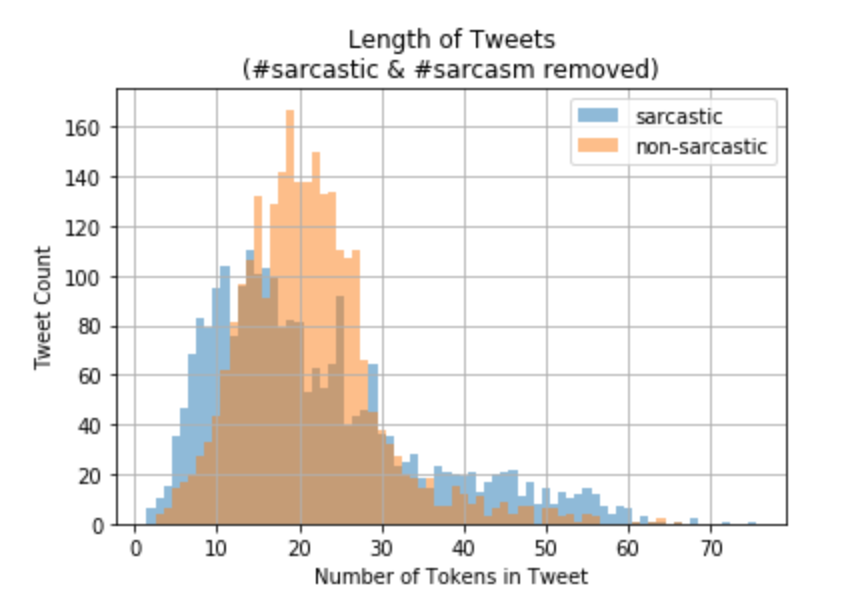
\includegraphics[width=75mm,scale=0.5]{token_histogram.png}

By comparing the distribution of tweet length for sarcastic and non-sarcastic tweets, we see that there is a right skew in the sarcastic distribution. The higher number of tweets with fewer tokens for the sarcastic class may be indicative of there being more meaning grounded in context being referenced to--as we might see in the distribution of sarcastic tweets with context below. The tweet length for non-sarcastic tweets is centered around 20 tokens and seem to be more normally distributed as we might expect from given that we use a large number of popular topic hashtags to represent the general population. We can see above that, generally speaking we can contain the full content of a tweet distilled into a set of 60 tokens (over 95\% of tweets contained less than 60 tokens). For the CNN model, we assumed a length of 40 tokens, allowing us to pad short tweets and short context with a "PADDING" tokens to ensure consistent tweet length. Tweets longer than 40 tokens were truncated. This means that sarcastic tweets were more likely affected by this methodological decision.

Next we reviewed the hashtag counts. 

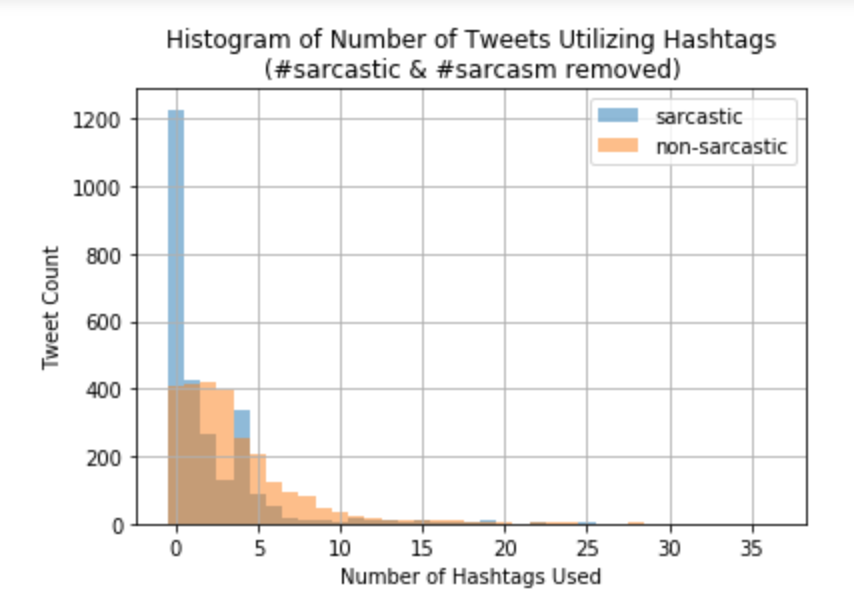
\includegraphics[width=75mm,scale=0.5]{hashtag_histogram.png}

We see that for sarcastic tweets there is a right-skewed in the distribution of number of hashtags utilized/referenced in a given tweet. This means that for any sarcastic tweets, we expect the user will be less likely to utilize additional tweets to accompany the \#sarcasm and/or \#sarcastic hashtags . In the non-sarcastic distribution there is less of a skew in the distribution with a median value around 4 hashtags in a tweet. We can see that in general, non sarcastic tweets are more likely to include hashtags for words other than the ones we used to sample our data. 

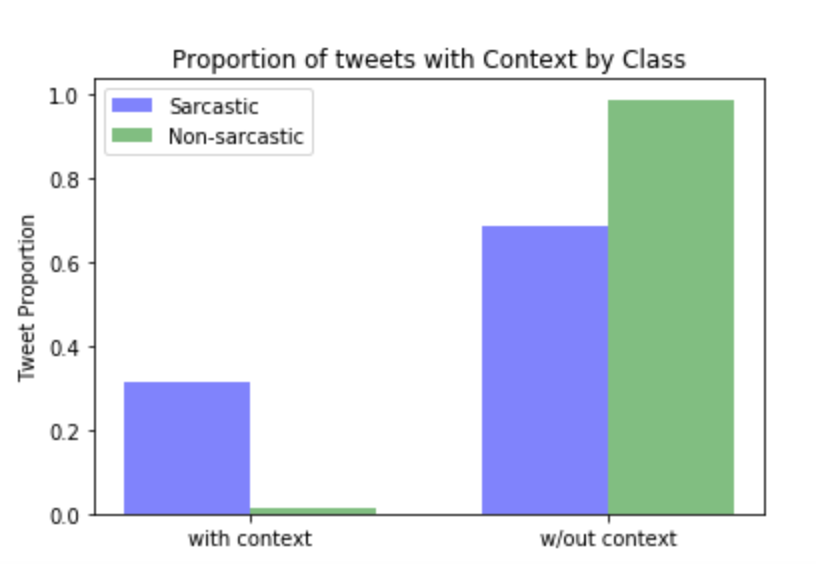
\includegraphics[width=75mm,scale=0.5]{context_proportion.png}

The bar chart above shows that both for sarcastic and non-sarcastic tweet have a larger proportion of tweets that are not in response to a preceding tweet in a message thread.  However, when looking at the left group of bars showing those proportions of the each of the two classes of tweets that have context, we see that there is a much higher percentage of sarcastic tweets with context than non-sarcastic tweets.

\subsection{Defining our Vocabulary}

To define our vocabulary we took two main approaches. The key difference in the approach was the treatment of hashtags. In one version, hashtags were tokenized as separate tokens. This allows us to capture additional context that may not be available in using only the prior tweet. To confirm that this methodology helped improve accuracy of our model, we also mapped all hashtags to a single token, which we named "HASHTAG". 

Under both methodologies, we tokenized all URLs as "LINK" tokens, retweet tags (including username attached to that retweet as "retweet", all remaining usernames as "USERNAMES", and finally each digit in a number as DG. 

We tuned the vocabulary length using the CNN model to decide on optimal vocabulary size. To that end, we found that a vocabulary of only 5,000 words was optimal. This is likely driven by the relatively small size of the dataset we built. With a larger dataset, we'll likely be able to improve the accuracy of our models with a larger vocabulary as we will be less likely to run into overfitting issues.

\subsection{Baseline}
A baseline model was built using a word count based multinomial Naive Bayes bag of words model with Laplace smoothing. The bag of words used was defined using the methodology described above. 

The multinomial Naive Bayes model uses an alpha of 0.1, meaning that we add a count of 0.1 to each word to ensure that we do not predict 0 probability for infrequently observed words. A series of alphas was tested using cross-validation but 0.1 proved to be optimal for our data set.

\subsection{Bi Convolutional Neural Network Model}

A model was implemented that uses an architecture proposed by Yin et. al [5]. The model is as follows. Two separate CNN processes are run where one processes the context sentence and the other processes the tweet of interest. An embedding layer generates an embedding vector for each token in our vocabulary. This embedding layer is shared between the two CNN processes. We opted against pre-trained word vectors as we wanted to capture the dynamic nature of twitter tweets as well as generate word vectors for hashtags and emojis. 

Each set of word vectors is then concatenated together and is then passed through the convolutional layer. By padding our tweets, we effectively have what is a variation of the wide variation. This variation generates an embedding for the "PADDING" token instead of a 0 embedding. The convolution layer also allows for the sharing of the convolution weights across the two processes. A tanh activation function of the form tanh(W*c + b)  where c is the concatenated word vectors, W is the convolution weights, and b the bias is used. Similar to Yin et. al, we use an average pooling layer that results in a tweet embedding vector of the same size as the word embedding vectors. The two resulting tweet vectors are concatenated together, and a logistic regression output layer is applied to the concatenated word vectors.

A diagram describing this procedure is below.

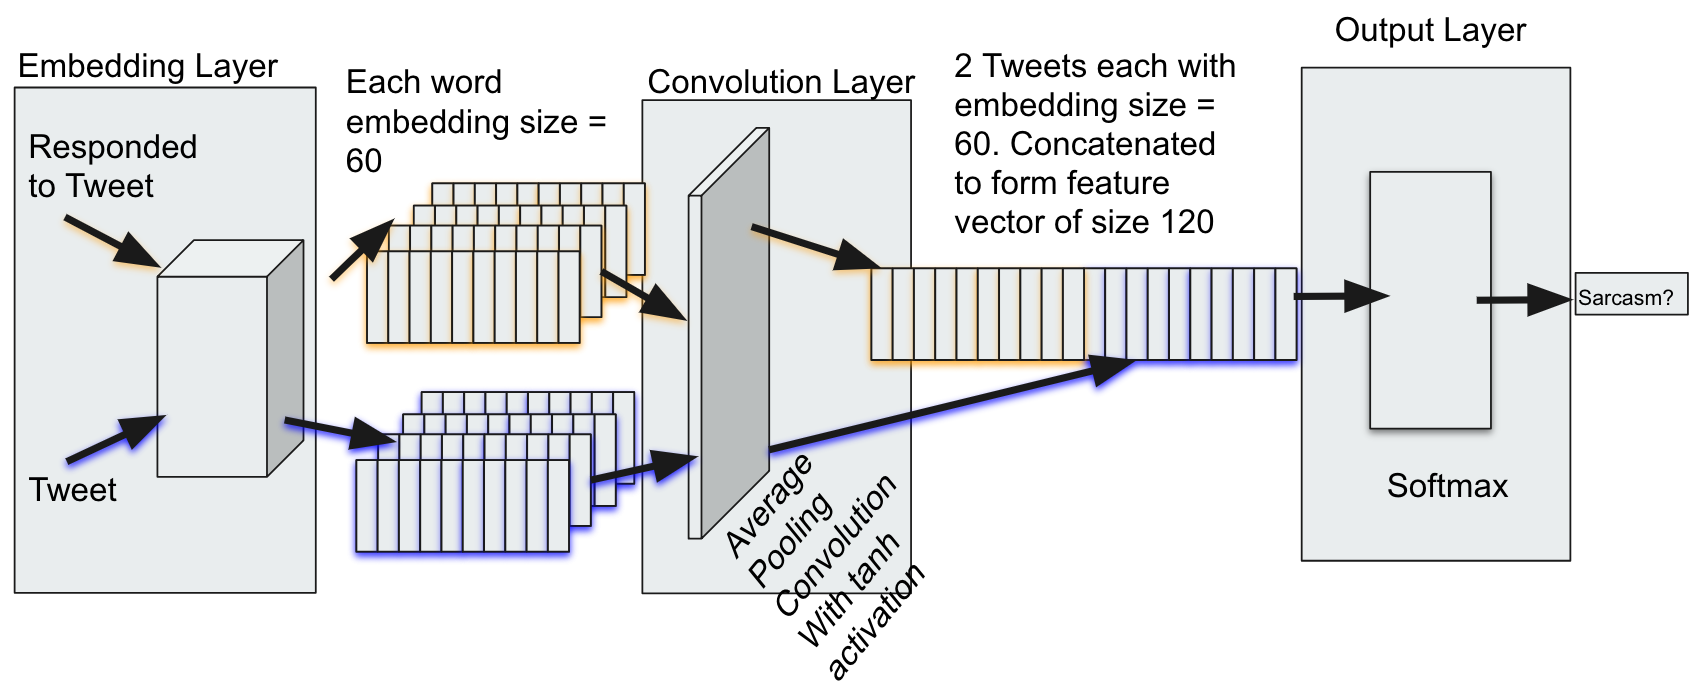
\includegraphics[width=75mm,scale=0.5]{bcnn.png}

The implementation of the algorithm that we rely on in this paper is using an embedding vector size of 60, a dropout keep probability of 40\%, a batch size of 200, using 10 epochs and no L2 regularization, which we determined using a series of cross validation tests.

\section{Results and Error Analysis}

A comparison of the different models we built as well as the best models proposed by the authors discussed in the background research section can be seen below.

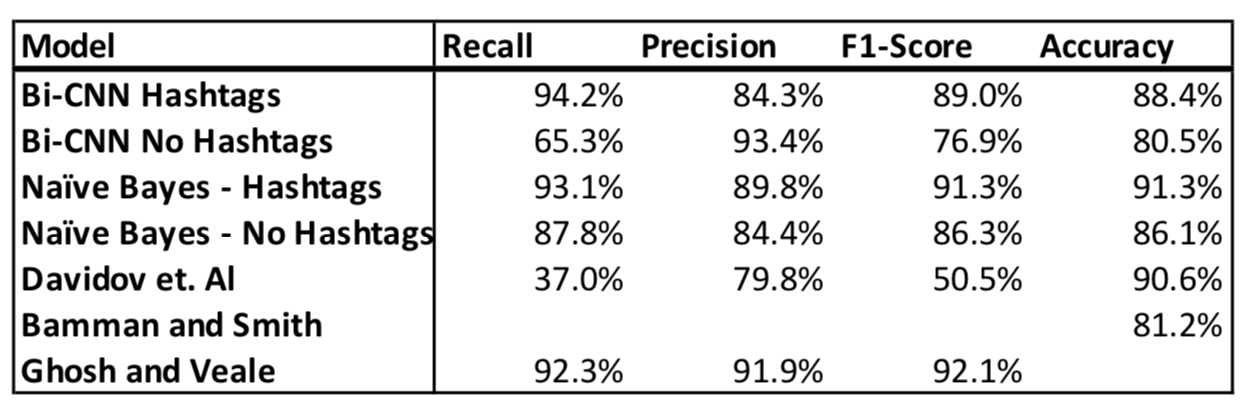
\includegraphics[width=75mm,scale=0.5]{results.png}

Our Naive Bayes algorithm outperformed our Bi CNN model as well as most of the works presented by the authors described.

To check for common errors, we randomly sampled from the top  tweets that our model got wrong. The method for this was simple. For the CNN model we looked at the difference in the logits and ranked each tweet this way, while for the Naive Bayes model we used the differences int he log probabilities. 

One common error mostly present in all models is the classification of . It seemed to consider compliments as sarcastic. Likely, what this shows is that compliments in twitter are rare, and when a compliment is seemingly made of someone, it is sarcastic. 

As described in our EDA section, non-sarcastic tweets were much more likely to heavily use hashtags. For this reason the models which mapped all hashtags to a single "HASHTAG" token were overconfident in tweets where a large number of hashtags were present in the tweet, an issue we attempted to remedy by mapping each hashtag to its own token. By giving each token its independent token, we were able to make our Naive Bayes model substantially less overconfident in tweets it got wrong while also becoming more accurate. Similar accuracy gains were achieved with the BCNN model when we tokenized hashtags independently, but the model had issues in being overconfident in tweets it classified incorrectly. In both cases the Naive Bayes model outperformed our BCNN model. However despite these adjustments, hashtag heavy tweets continued to have a high frequency of being tagged as non-sarcastic.

It's unsurprising that our Naive Bayes models outperformed our BiCNN models. This is likely because our data set was relatively small, and we relied on relatively small word embedding sizes. Furthermore, the Naive Bayes algorithm is able to simply identify the hashtags that were used to generate the negative samples. Still the model continued to perform extremely well on the test set even without keeping the hashtags as their own separate token. However, we believe that this is likely driven by the fact that our models might simply be picking up words idiosyncratic to the hashtags we used to generate our negative examples, and thus may not be properly learning to distinguish what sarcasm is. That is, our algorithms may simply be learning words that describe the hashtags we used to generate our negative example data set. 

\section{Additional Observations}

Some interesting patterns emerged within our data. For instance, we uncovered certain emojis were tagged as heavily sarcastic. These emojis are below:

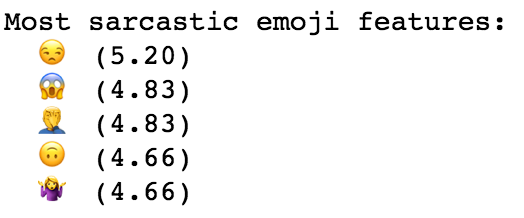
\includegraphics[width=75mm,scale=0.5]{top_emoji.png}

The emojis that were tagged as most sarcastic are not too surprising, which shows that the Naive Bayes model is picking on interesting linguistic phenomena. As described in the error analysis, the CNN model seems to be picking up on similar phenomena within emojis, because as we noted, one of the most overconfident errors that our CNN model was likely driven heavily by the use of one of these emoji.

A few hashtags were also present in the positive examples, most had a humor theme, such as \#jokes, \#puns, \#funnyquotes, \#oneliner, \#snarky. This is to be expected. Likely, to dampen the impact of sarcasm, users would follow their message with a signal letting others know that their message was made in good fun.

\section{Conclusion}

We began by implementing a multinomial Naive Bayes model with Laplace smoothing. This model resulted in surprisingly accurate predictions. 

We then implemented the  Bi-CNN model, which encodes sarcasm using two separate sentences, the tweet that our tweet of interest is responding to as well as the tweet of interest itself. This allows us to forego the use of user embeddings while still building context, without a significant loss of accuracy compared to the models described by other authors. Due to the size of the data used, this model did not perform as well as the Naive Bayes, but we're confident that more training data will tip the scales toward the Bi-CNN.  

One important caveat of our methodology is that our data is likely heavily overfitting to the context which we collected our non-sarcastic training data. Regardless, we still uncovered interesting phenomena within the sarcastic hashtags and emojis.

We're confident that with better sampling methodology and a much larger data set, this algorithm will continue to improve on its ability to pick up on sarcastic cues.  Adding the attention mechanism discussed by Yin et. will likely improve on the methodology even more.

\section{Special Thanks}

We'd like to give special thanks to Denny Britz for writing a very helpful guide on implementing a CNN in TensorFlow. We relied heavily on his code to build our BiCNN model. [6]

\textbf{References}

[1] http://www.aclweb.org/anthology/W10-2914

[2] https://homes.cs.washington.edu/~nasmith/papers/bamman+smith.icwsm15.pdf

[3] https://arxiv.org/pdf/1607.00976v2.pdf

[4] http://www.aclweb.org/anthology/W16-0425

[5] https://arxiv.org/pdf/1512.05193v3.pdf

[6] http://www.wildml.com/2015/12/implementing-a-cnn-for-text-classification-in-tensorflow/

\end{document}
